\newcommand{\CifarDatasetSlide}{
\begin{columns}[T]
  \column{\customcolumnwidth}
    \textbf{Dataset Characteristics}
    \begin{itemize}
      \item 60,000 RGB images (32x32 pixels)
      \item 10 \emph{balanced} categories
      \item Standard split:
      \begin{itemize}
        \item 50,000 training
        \item 10,000 test (1,000/class)
      \end{itemize}
      % \item Categories:
      % \begin{itemize}
      %   \item Natural: birds, cats, deer, dogs, frogs, horses
      %   \item Artificial: airplanes, automobiles, ships, trucks
      % \end{itemize}
      \item \emph{Common} vision task
    \end{itemize}
  \column{\customcolumnwidth}
    \begin{figure}
    % CIFAR-10 examples figure
\begin{figure}[h]
  \begin{tabular}{ccccc}
    \begin{minipage}[b]{0.15\linewidth}
      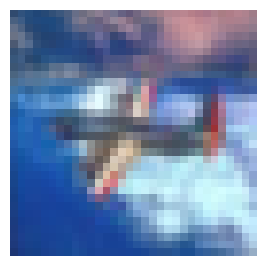
\includegraphics[width=\linewidth]{figures/cifar-images/airplane.png}
      \centering\scriptsize\texttt{airplane}
    \end{minipage} &
    \begin{minipage}[b]{0.15\linewidth}
      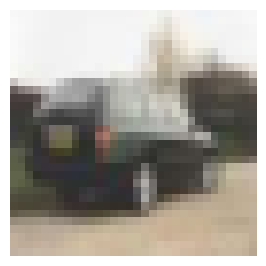
\includegraphics[width=\linewidth]{figures/cifar-images/automobile.png}
      \centering\scriptsize\texttt{auto}
    \end{minipage} &
    \begin{minipage}[b]{0.15\linewidth}
      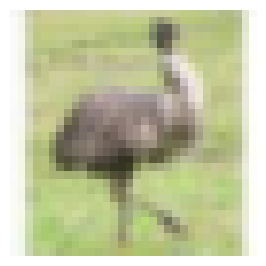
\includegraphics[width=\linewidth]{figures/cifar-images/bird.png}
      \centering\scriptsize\texttt{bird}
    \end{minipage} &
    \begin{minipage}[b]{0.15\linewidth}
      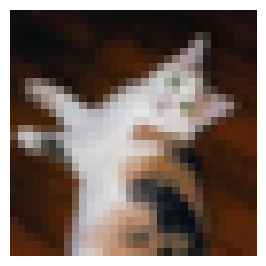
\includegraphics[width=\linewidth]{figures/cifar-images/cat.png}
      \centering\scriptsize\texttt{cat}
    \end{minipage} &
    \begin{minipage}[b]{0.15\linewidth}
      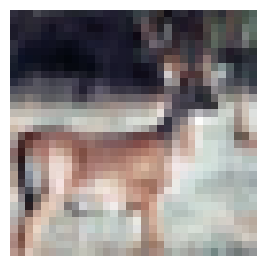
\includegraphics[width=\linewidth]{figures/cifar-images/deer.png}
      \centering\scriptsize\texttt{deer}
    \end{minipage} \\
    \begin{minipage}[b]{0.15\linewidth}
      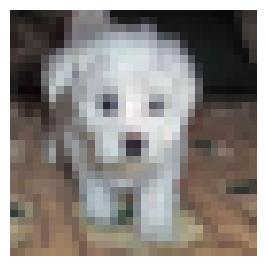
\includegraphics[width=\linewidth]{figures/cifar-images/dog.png}
      \centering\scriptsize\texttt{dog}
    \end{minipage} &
    \begin{minipage}[b]{0.15\linewidth}
      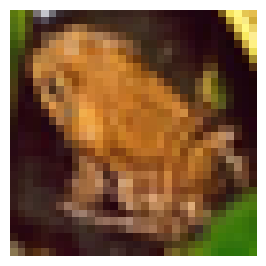
\includegraphics[width=\linewidth]{figures/cifar-images/frog.png}
      \centering\scriptsize\texttt{frog}
    \end{minipage} &
    \begin{minipage}[b]{0.15\linewidth}
      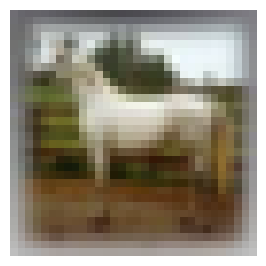
\includegraphics[width=\linewidth]{figures/cifar-images/horse.png}
      \centering\scriptsize\texttt{horse}
    \end{minipage} &
    \begin{minipage}[b]{0.15\linewidth}
      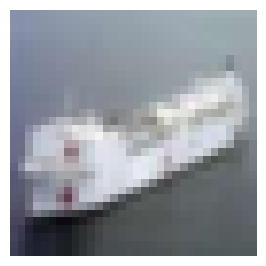
\includegraphics[width=\linewidth]{figures/cifar-images/ship.png}
      \centering\scriptsize\texttt{ship}
    \end{minipage} &
    \begin{minipage}[b]{0.15\linewidth}
      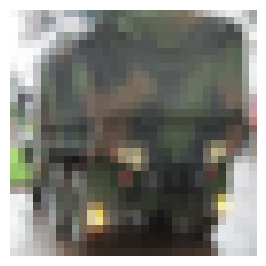
\includegraphics[width=\linewidth]{figures/cifar-images/truck.png}
      \centering\scriptsize\texttt{truck}
    \end{minipage}
  \end{tabular} 
\end{figure}
    \caption{Example images from CIFAR-10~\footfullciteieee{Krizhevsky2009}}
    \end{figure}
\end{columns}
}